\appendix

\chapter{Mixed-Integer Programming Formulation details}

\section{Feasibility constraints.\label{appendix:feasibility_constr}}
We denote $\mathcal{F}$ the set of kinematic and dynamic feasibility constraints, as explained in \cite{sl1m_v1}. 
It includes some constraints on the robot center of mass for its equilibrium and the reachability of the planned contacts.
As a result, they guarantee the feasibility of the robot contacts, which are characterized by their position $p$ and orientation $r$.

\paragraph{Center of mass constraints}
\begin{figure}[t]
    \centering
    \captionsetup[subfigure]{justification=centering}
    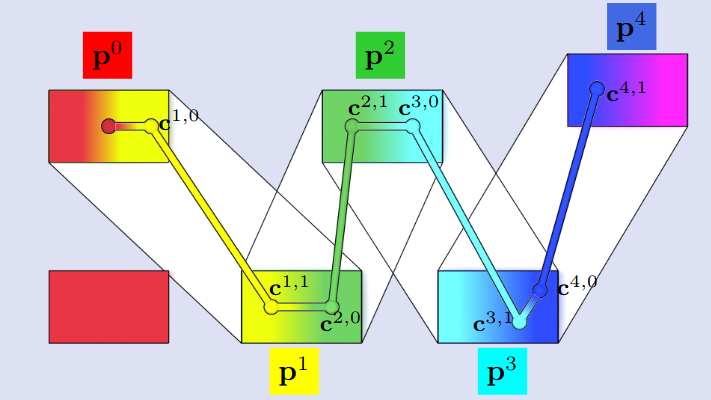
\includegraphics[width=0.8\textwidth]{Figures/Appendix/2pac_feasibility.png}
    \caption{Computation of a feasible center of mass quasi-static trajectory using the 2PAC method \cite{Tonneau2018_2PAC}. Source: Tonneau et al. \cite{sl1m_v1}}
    \label{fig:mip:feasibility_constr}
\end{figure}
We guarantee the equilibrium and balance constraints using the 2PAC formulation \cite{Tonneau2018_2PAC}.
These constraints will be succintly explained and we refer the reader to \cite{sl1m_v1} for further details.
Using this formulation, we only need to select 2 Center Of Mass (COM) positions for each phase $k$ from step $p_{k-1}$ to $p_k$, that are $c_{k,\:0}$ and $c_{k,\:1}$ to guarantee continuous feasibility (Figure \ref{fig:mip:feasibility_constr}).

In the context of biped walking, a sufficient condition for static equilibrium is to ensure that the center of mass lies above the support effector.
The constraint can be formulated as follows:
\begin{equation}
    \label{eq:equilibrium_constr}
    \begin{aligned}
        F_{k-1} (c_{k,\:0}-p_{k-1}) &\leq  f_{k-1}\\% + M a_{k-1}^{j}\\
        F_{k} (c_{k,\:1}-p_{k}) &\leq  f_{k}% + M a{k}^{j}
    \end{aligned}
\end{equation}
where $F_k$ and $f_k$ are the matrix and vector defining the polygonal shape of the foot at $p_k$ (considering the contact lies on flat ground).
Constraints (\ref{eq:equilibrium_constr}) depends only on the xy coordinates of the COM.
As a result, by convexity of the static equilibrium regions, the straight lines $[c_{k,\:0}, c_{k,\:1}]$ continuously satisfies the static equilibrium
constraint, as well as $[c_{k-1,\:1}, c_{k,\:0}]$ and $[c_{k,\:1}, c_{k+1,\:0}]$ as the COM stays above the corresponding support effector.

\paragraph{Reachability constraints.}
We also use the center of mass positions $c_{k,\:0}$ and $c_{k,\:1}$ to guarantee kinematic reachability.
A 3D polytope $\mathcal{R}$ is obtained for each effector (feet in our case) via offline random sampling, approximating the reachable COM workspace.
The resulting polytope is expressed as follows: $\mathcal{R} : \{c \in \mathbb{R}^3 , \; \! R c \; \leq \; \! r\}$.

For each phase $k$, we consider the orientation of the foot frame constant and equal to $r_{k-1}$.
We note $\mathcal{R}_k$ the rotated polytope associated with contact $p_{k}$.
For phase $k$, the contraints on the COM positions $c_{k,\:0}$ and $c_{k,\:1}$ can be formulated as follows:
\begin{equation}
    %R_{l}^j (c_{l,e} - p_{l}) \leq r_l^j + M a_l^j \;\;\;\; \forall j, \forall l \in \{k-1,k\}
    R_{l} (c_{l,e} - p_{l}) \leq r_l \;\;\;\; \forall l \in \{k-1,k\}
\end{equation}

\paragraph{Relative foot position constraints.\label{appendix:foot_pos_constr}}
Just as for the COM reachability, a 3D polytope $\mathcal{Q}$ is randomly sampled offline (or manually given) to approximate the reachable workspace of each foot with respect to the other. The polytope rotated by $r_{k-1}$ then translated by $p_{k-1}$ can be expressed as $\mathcal{Q}_k: \{ p \in \mathbb{R}^3, Q_k p \leq q_k \}$.
For phase $k$, the relative foot position constraints can be formulated as follows:
\begin{equation}
    %\mathcal{Q}_{k-1}^j (p_k - p_{k-1}) \leq q_{k-1}^j + M a_{k-1}^j \;\;\;\; \forall j
    \mathcal{Q}_{k-1} (p_k - p_{k-1}) \leq q_{k-1}
\end{equation}

\section{Complete MIP Formulation \label{appendix:complete_mip_formulation}}
The complete formulation of the contact-before-motion MIP contact planning problem with the center of mass positions and the feasibility constraints of previous Appendix \ref{appendix:feasibility_constr} is:

\begin{align}
    \textrm{\textbf{given}} %\quad & \mathcal{I}=\{p_0^{left}, r_0^{left},p_0^{right}, r_0^{right}\} \nonumber\\
    %\textrm{, the initial foot position}\\
                            %\quad & n\\%\textrm{, the desired number of contacts}\\
                            %\quad & \mathcal{S}=\{\mathcal{S}^0,...,\mathcal{S}^m\}\\%\textrm{, the set of terrain surfaces}\\
                            %\quad & \mathcal{S}^{goal}\\%\textrm{, the goal surface to reach}\\
                            \quad & n, \; p_0, \; r_0, \; \mathcal{S}, \; \mathcal{S}^{goal} \nonumber\\
    \textrm{\textbf{find}}  \quad & P=[p_1,...,p_n], \; p_i \in \mathbb{R}^{3 \times n} \nonumber\\
                            \quad & R=[r_1,...,r_n], \; r_i \in \mathbb{R}^{3 \times n} \nonumber\\
                            \quad & \textcolor{blue}{C=[c_{0,1},c_{1,0},c_{1,1},...,c_{n,0},c_{n,1}]}, \; c_{k,e} \in \mathbb{R}^3 \nonumber\\
                            \quad & A=[a_1,...,a_n], \; a_i \in \{0,1\}^{m} \nonumber\\
                            \quad & \beta=[\beta_1,...,\beta_n], \; \beta_i \in \mathbb{R}^{m} \nonumber\\
                            %\quad & \alpha=[\alpha_1,...,\alpha_n] \in \mathbb{R}_{+}^{n}\\
    %\min_{w,b,\xi} \quad & \frac{1}{2}w^{t}w+C\sum_{i=1}^{N}{\xi_{i}}\\
    \textrm{\textbf{min}}  \quad & l(P,R,\textcolor{blue}{C}) \nonumber\\
    \textrm{\textbf{s.t.}}  \quad & p_n \in \mathcal{S}^{goal} \nonumber\\
                            \quad & \forall i \in \{1,..,n\} : \nonumber\\
                                \quad & \quad \sum_{j=1}^{m} a_i^j = m-1  \nonumber\\
                                \quad & \quad \forall j \in \{1,..,m\} : \nonumber\\
                                    \quad & \quad \quad S^j p_i \leq s^j + M a_i^j  \nonumber\\
                                    \quad & \quad \quad (p_i)^{\intercal} \textbf{n}^j = e^j + \beta_i^j \nonumber\\
                                    \quad & \quad \quad ||\beta_i^j||_1 \leq M a_i^j \nonumber\\
                                    %\quad & \quad \quad \textcolor{blue}{F^{j}_{i-1} (c_{i,\:0}-p_{i-1}) \leq  f_{i-1}^{j} + M a_{i-1}^{j} } \nonumber\\
                                    %\quad & \quad \quad \textcolor{blue}{F^{j}_{i} (c_{i,\:1}-p_{i}) \leq  f^j_{i} + M a{i}^{j} }  \nonumber\\
                                    %\quad & \quad \quad \textcolor{blue}{R_{i}^j (c_{i,e} - p_{i}) \leq r_i^j + M a_i^j }  \nonumber\\
                                    %\quad & \quad \quad \textcolor{blue}{R_{i-1}^j (c_{i-1,e} - p_{i-1}) \leq r_{i-1}^j + M a_{i-1}^j } \nonumber\\
                                    %\quad & \quad \quad \textcolor{blue}{\mathcal{Q}_{i-1}^j (p_i - p_{i-1}) \leq q_{i-1}^j + M a_{i-1}^j} \nonumber
                                    \quad & \quad \quad \textcolor{blue}{F_{i-1} (c_{i,\:0}-p_{i-1}) \leq  f_{i-1}} \nonumber\\
                                    \quad & \quad \quad \textcolor{blue}{F_{i} (c_{i,\:1}-p_{i}) \leq  f_{i}}  \nonumber\\
                                    \quad & \quad \quad \textcolor{blue}{R_{i} (c_{i,e} - p_{i}) \leq r_i}  \nonumber\\
                                    \quad & \quad \quad \textcolor{blue}{R_{i-1} (c_{i-1,e} - p_{i-1}) \leq r_{i-1}} \nonumber\\
                                    \quad & \quad \quad \textcolor{blue}{\mathcal{Q}_{i-1} (p_i - p_{i-1}) \leq q_{i-1}} \nonumber
\end{align}